\documentclass[xcolor=dvipsnames,xcolor=table, 14p]{beamer}

% language support and encoding of input and output
\usepackage[english]{babel}
\usepackage[utf8]{inputenc}
% better font support
\usepackage[T1]{fontenc}
%\usepackage{lmodern}
\usepackage{avant} % URW gothic fonts
% graphical support
\usepackage[table]{xcolor}
\usepackage{graphicx}
% typographical improvement
\usepackage{microtype}
\usepackage{amsmath}
\usepackage{blkarray}
\usepackage{tikz}
\usetikzlibrary{arrows, positioning, automata}
\usepackage{csquotes}
\usepackage{booktabs}
\usepackage{subcaption}
\captionsetup[subfigure]{labelfont=rm}
\usepackage{caption}
\usepackage{listings}


\definecolor{codegray}{gray}{0.7}
\newcommand{\code}[1]{\colorbox{codegray}{\texttt{#1}}}

% define colors for background and text:
\definecolor{background}{HTML}{686262}
\definecolor{text}{HTML}{7abeff}
\definecolor{textalt}{HTML}{47a6ff}

% custom emphasize
\renewcommand{\emph}[1]{\textcolor{textalt}{\textbf{#1}}}
\newcommand{\mathemph}[1]{\textcolor{textalt}{\mathbf{#1}}}

% setting up Beamer theme and look
\usetheme{Madrid}
\setbeamertemplate{items}[circle]
\setbeamertemplate{blocks}[rounded][shadow=true]
\usecolortheme[named=background]{structure}
\setbeamertemplate{navigation symbols}{}

% For TOC
\setbeamertemplate{section in toc}[square]

\setbeamercolor{frametitle}{fg=text}
\setbeamercolor{title}{fg=text}
\setbeamercolor{subtitle}{fg=text}
\setbeamercolor{author}{fg=text}

\setbeamerfont{title}{series=\bfseries}
\setbeamerfont{frametitle}{series=\bfseries}
\setbeamerfont{author}{series=\bfseries}

% author and presentation information:
\author[J. M.]{Jiří Moravec}
% TODO title
\title[NZCD]{New Zealand Crash Data}
\date{}


\lstdefinestyle{codestyle}{
    backgroundcolor=\color{codegray},   
%    commentstyle=\color{codegreen},
%    keywordstyle=\color{magenta},
%    numberstyle=\tiny\color{codegray},
%    stringstyle=\color{codepurple},
    basicstyle=\ttfamily,
    breakatwhitespace=false,         
    breaklines=true,                 
    captionpos=b,                    
    keepspaces=true,                 
    numbers=none,                    
    numbersep=5pt,                  
    showspaces=false,                
    showstringspaces=false,
    showtabs=false,                  
    tabsize=4
    }

\lstset{style=codestyle}

\begin{document}

\begin{frame}
\maketitle
\end{frame}

\begin{frame}
Exploratory Data Analysis
\begin{itemize}
    \item full exploration of NZ Crash Data
    \item univariate and some bivariate relationships
    \item small modelling for relationship of interest
    \item code: \url{github.com/j-moravec/CrashDataEda}
    \item used CSV, but plugging REST API is not an issue
\end{itemize}

Limitations:
\begin{itemize}
    \item No expert / key available
    \item Limited time
\end{itemize}
\end{frame}

\begin{frame}
    \centering
    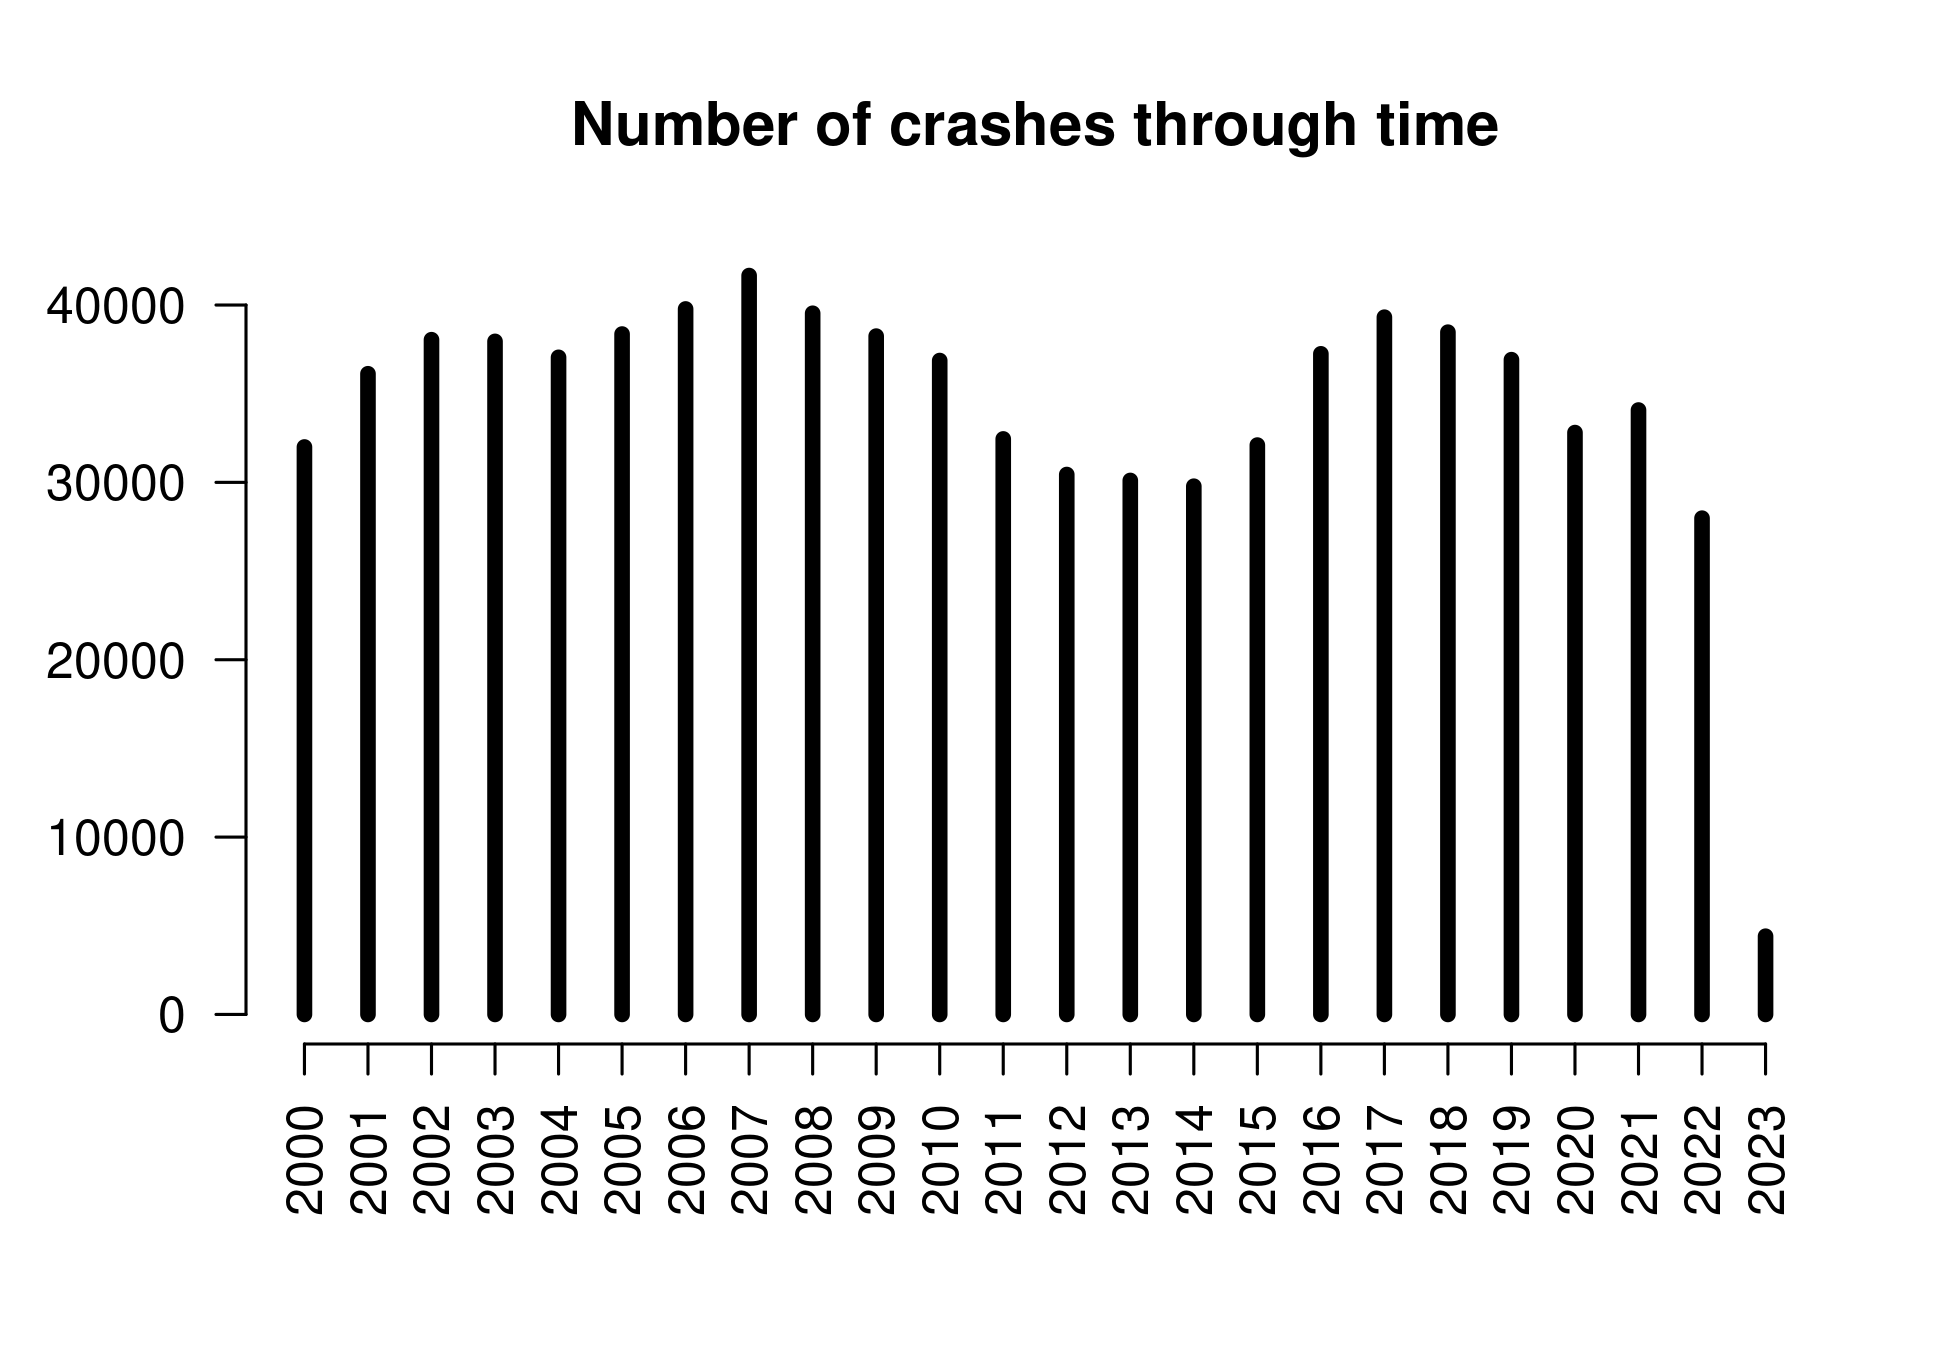
\includegraphics[width=1\textwidth]{figures/time-1.png}
\end{frame}

\begin{frame}
    \centering
    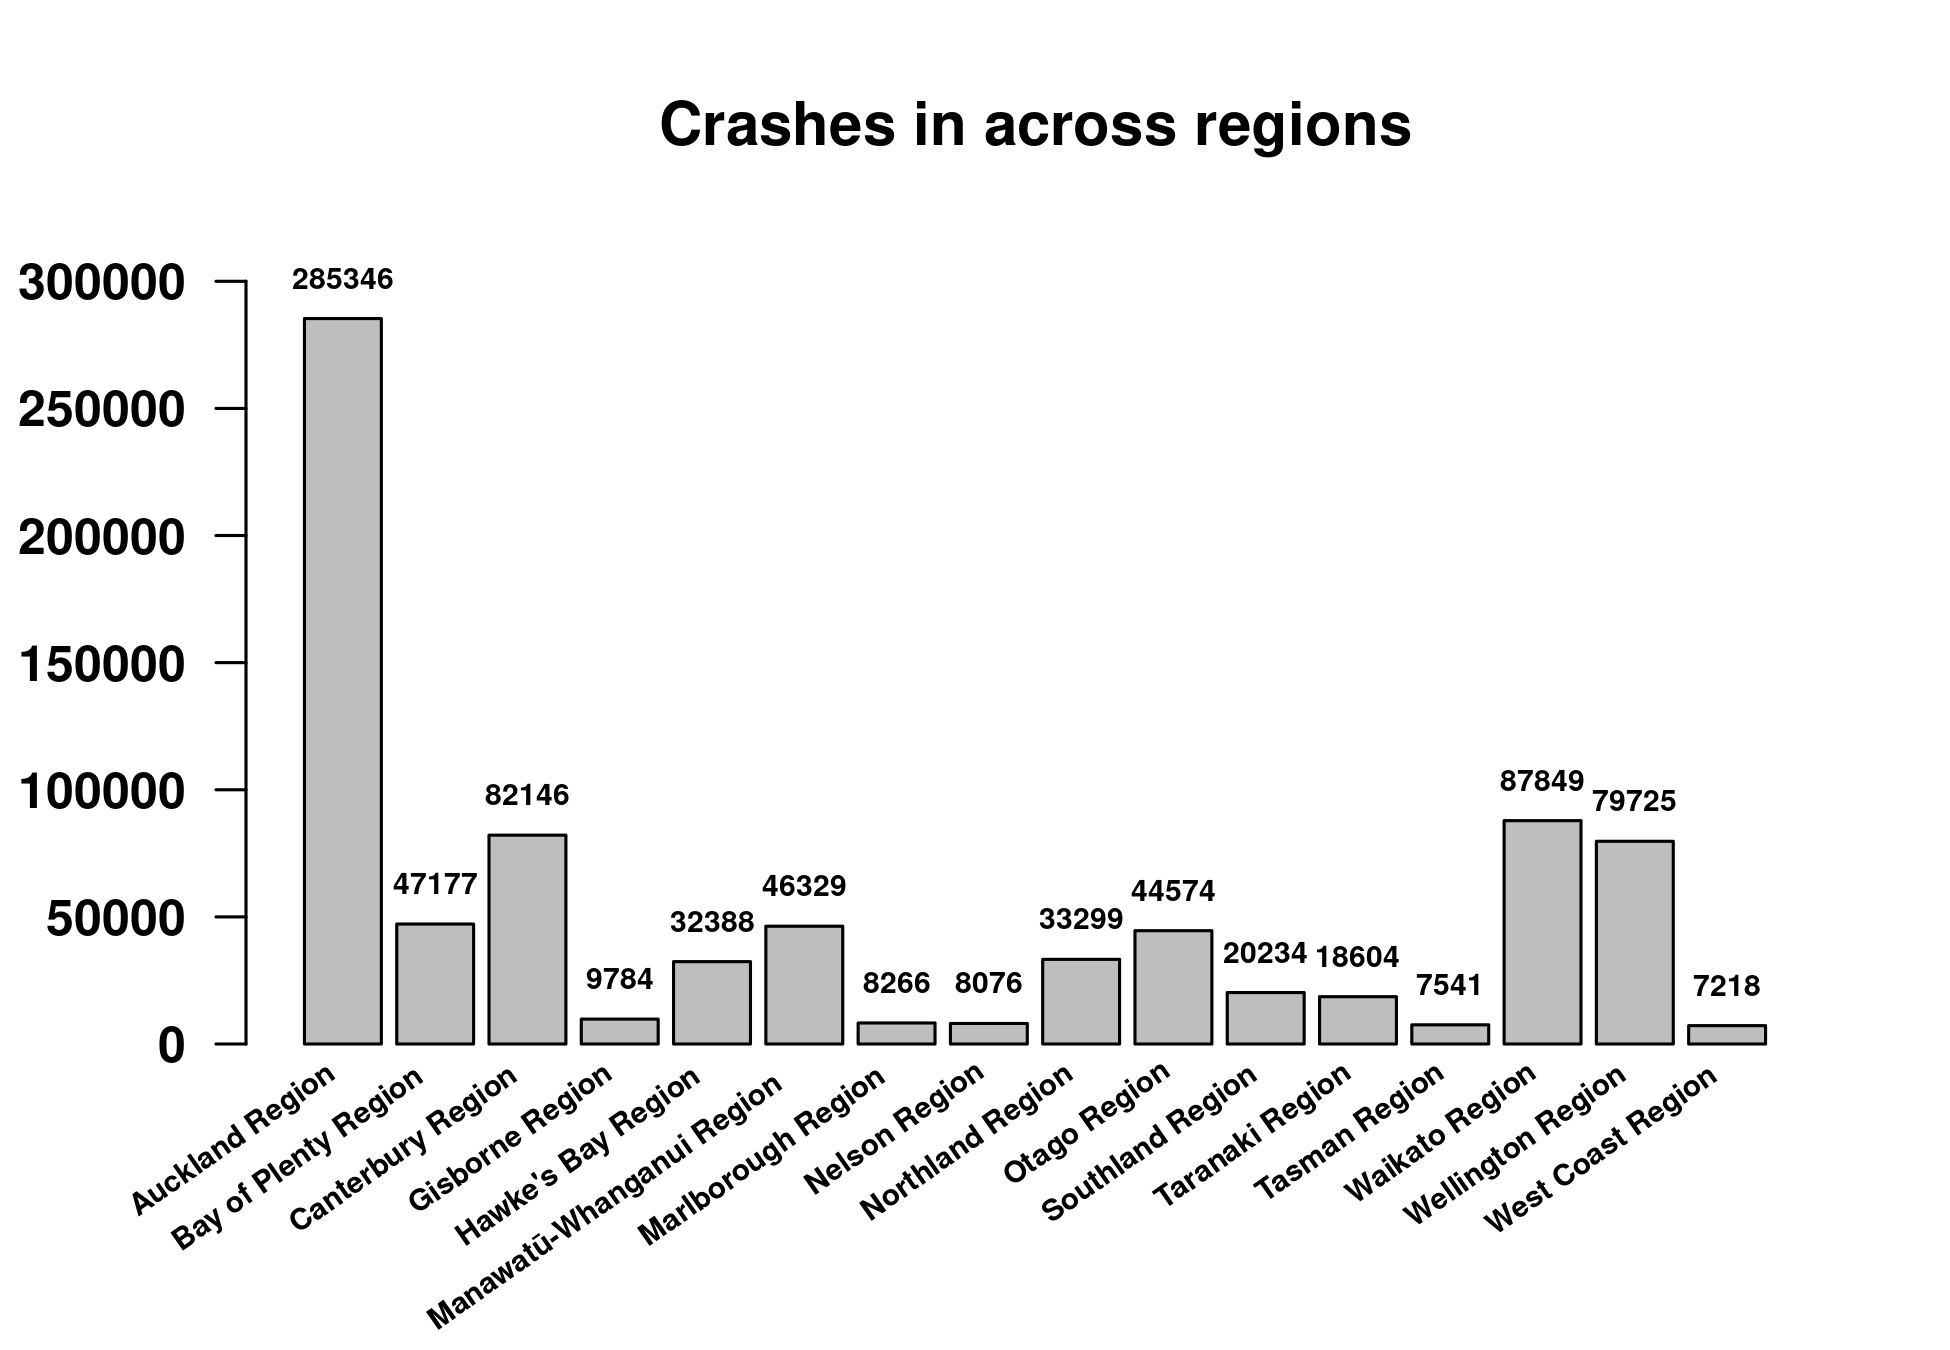
\includegraphics[width=1\textwidth]{figures/location2-1.png}
\end{frame}

\begin{frame}
    \centering
    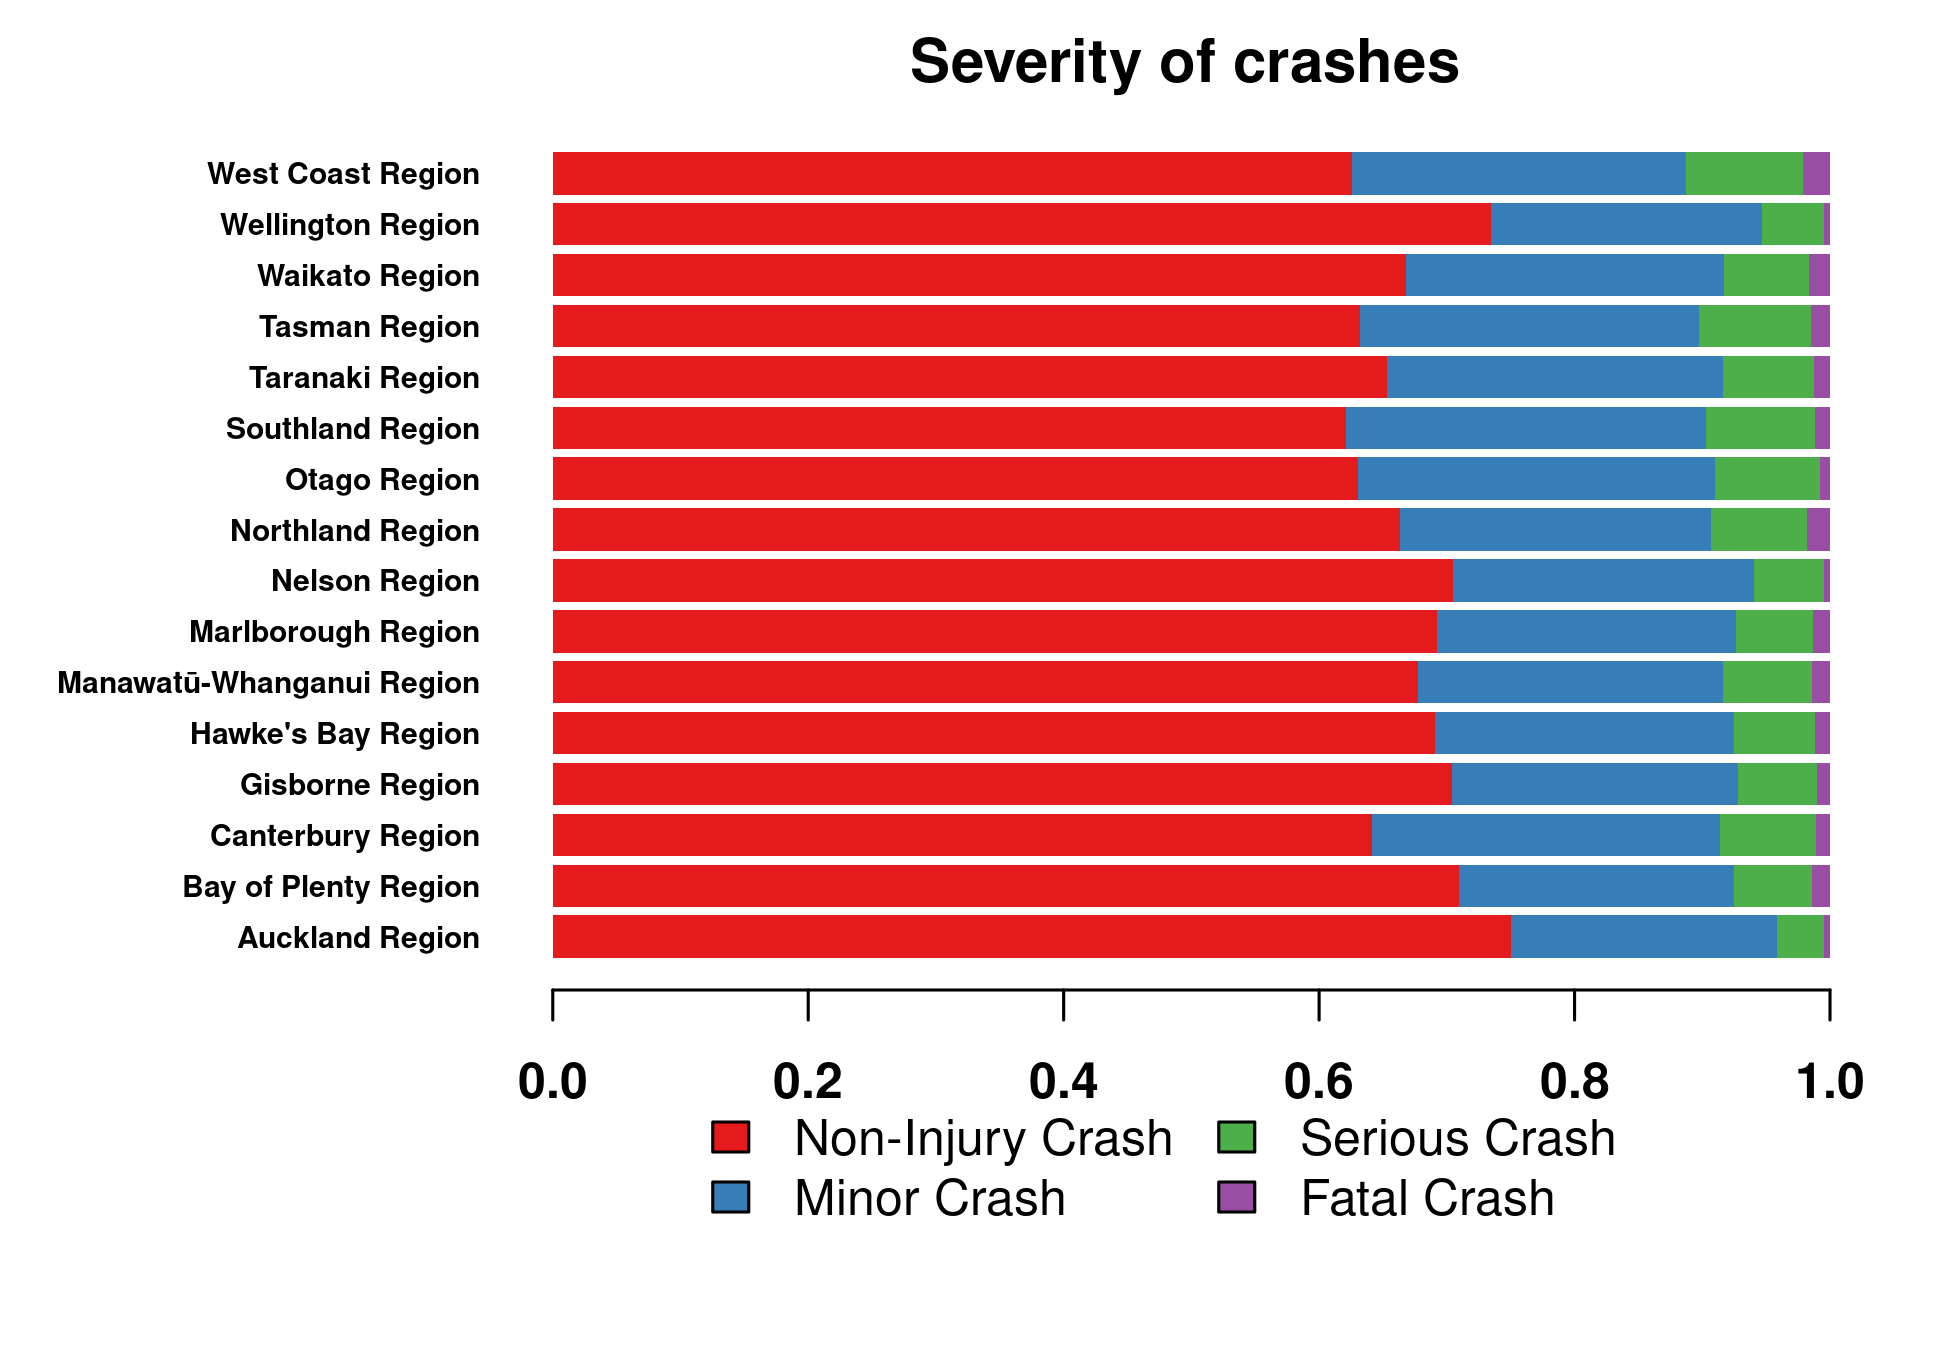
\includegraphics[width=1\textwidth]{figures/regions-1.png}
\end{frame}

\begin{frame}
    \centering
    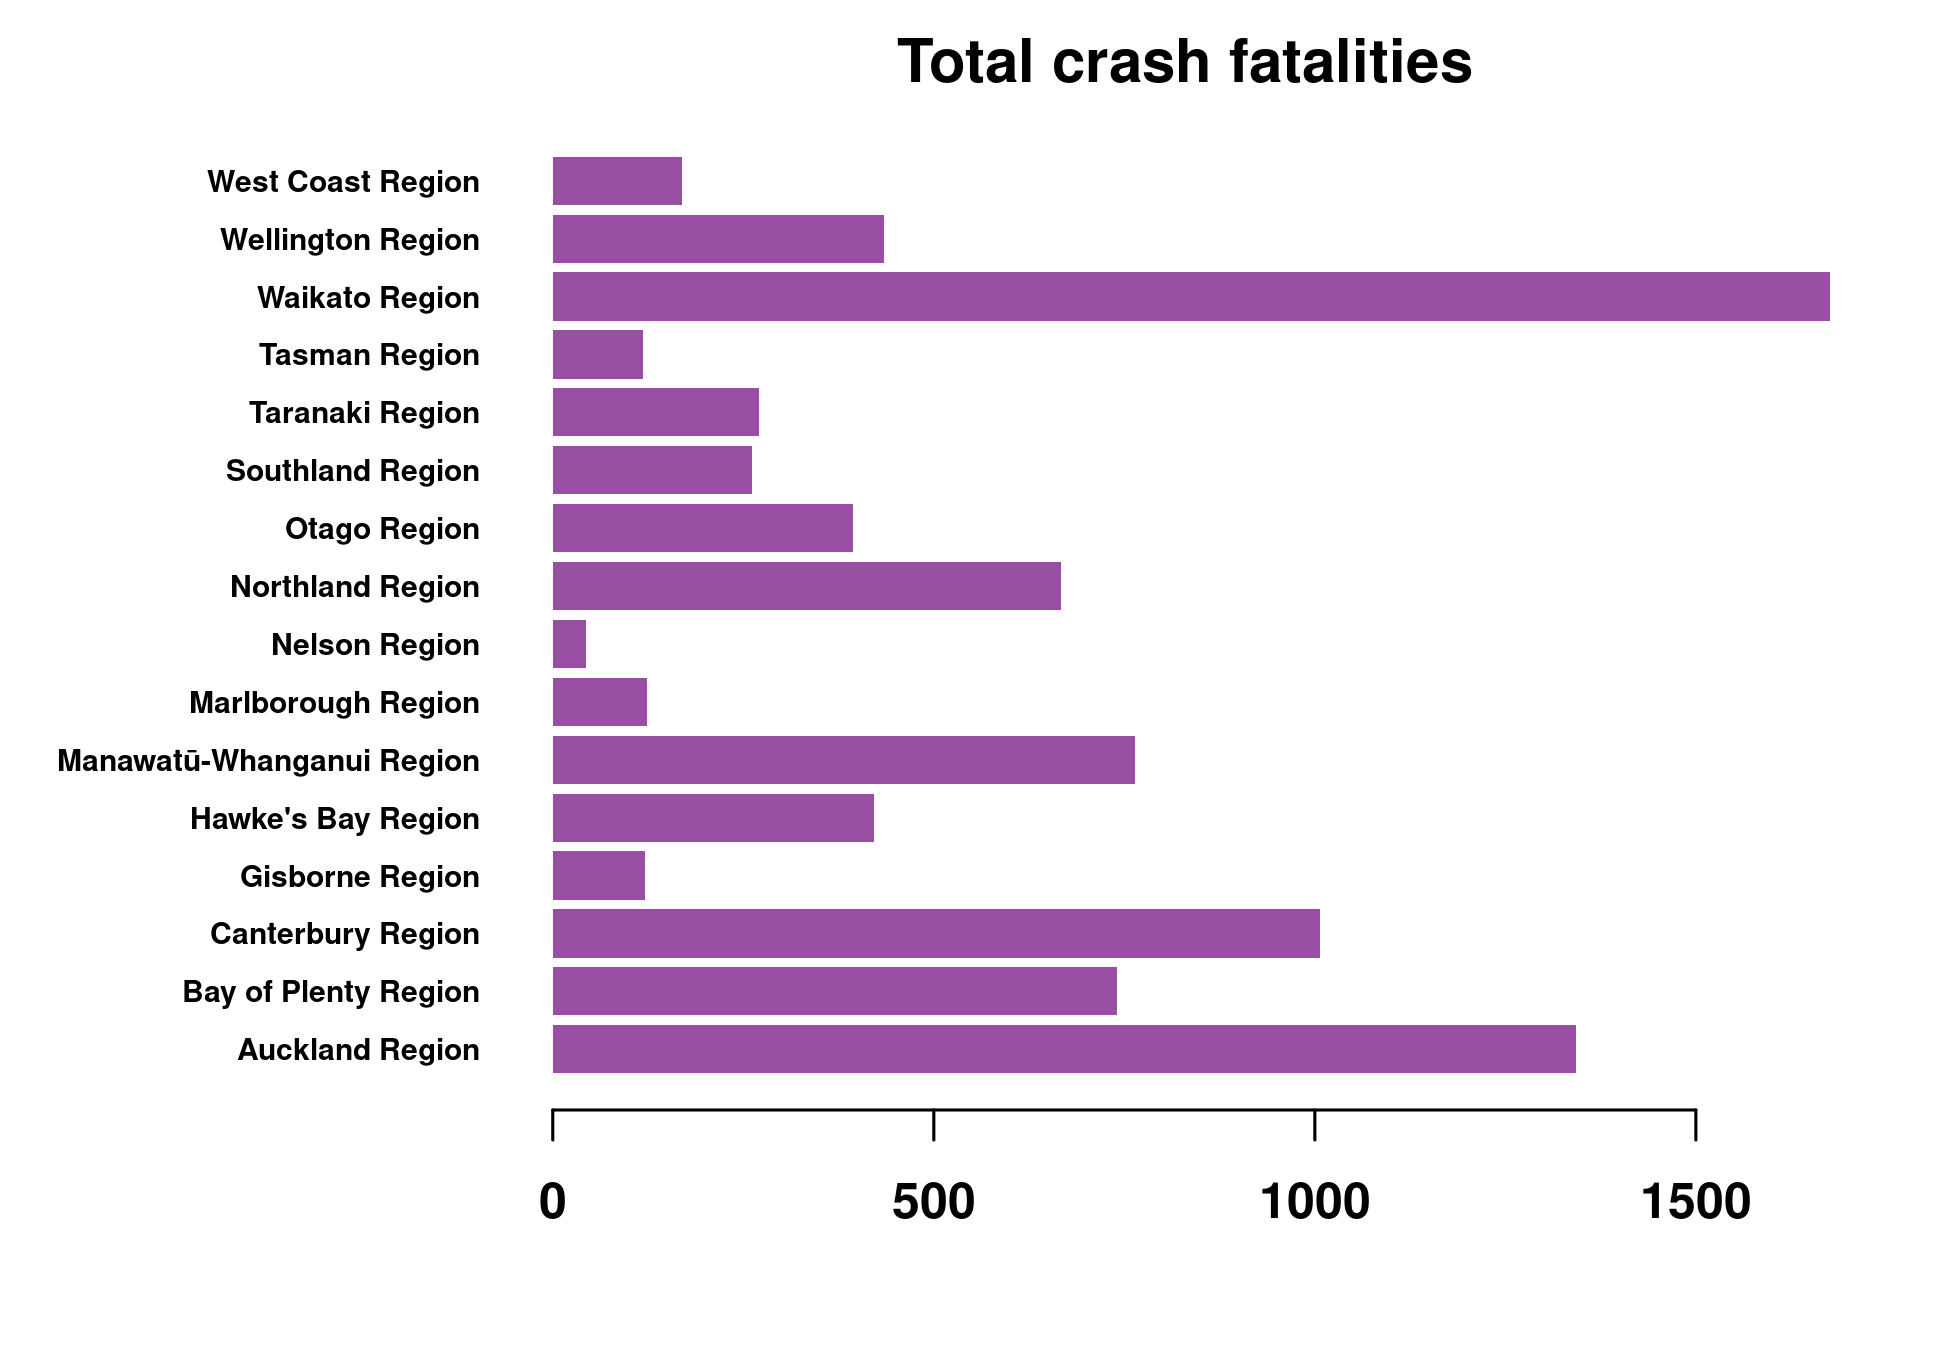
\includegraphics[width=1\textwidth]{figures/regions2-1.png}
\end{frame}

\begin{frame}
    \begin{columns}
        \begin{column}{0.5\textwidth}
        \begin{itemize}
            \item Variable: Crash severity
            \item Used models: CART, RandomForest
            \item Result: Failure
        \end{itemize}
        \end{column}

        \begin{column}{0.5\textwidth}
            \centering
            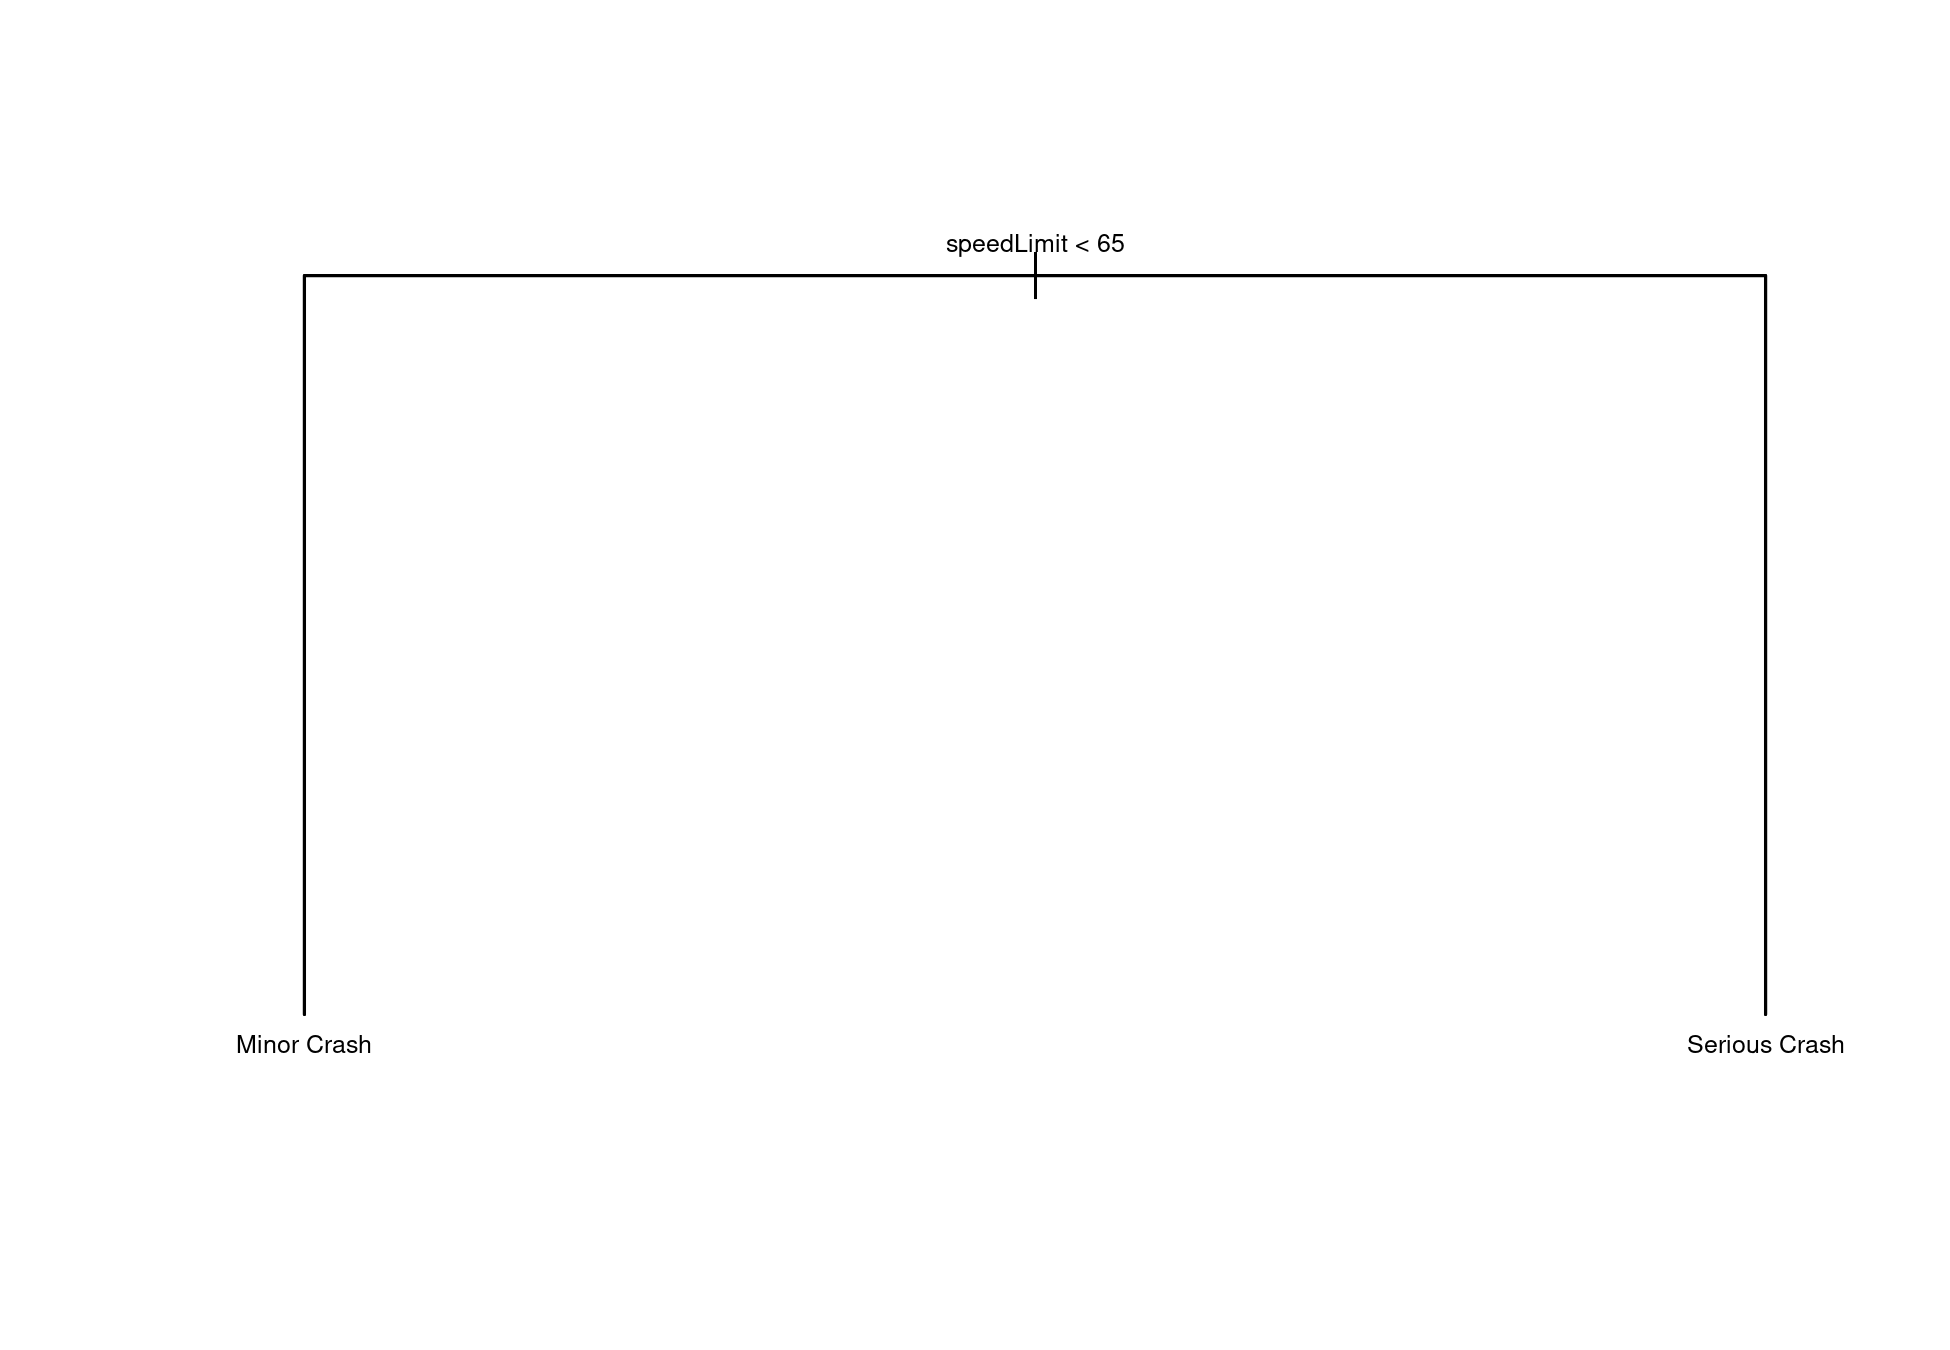
\includegraphics[width=1\textwidth]{figures/cart-1.png}
        \end{column}
    \end{columns}
\end{frame}

\begin{frame}
    \centering
    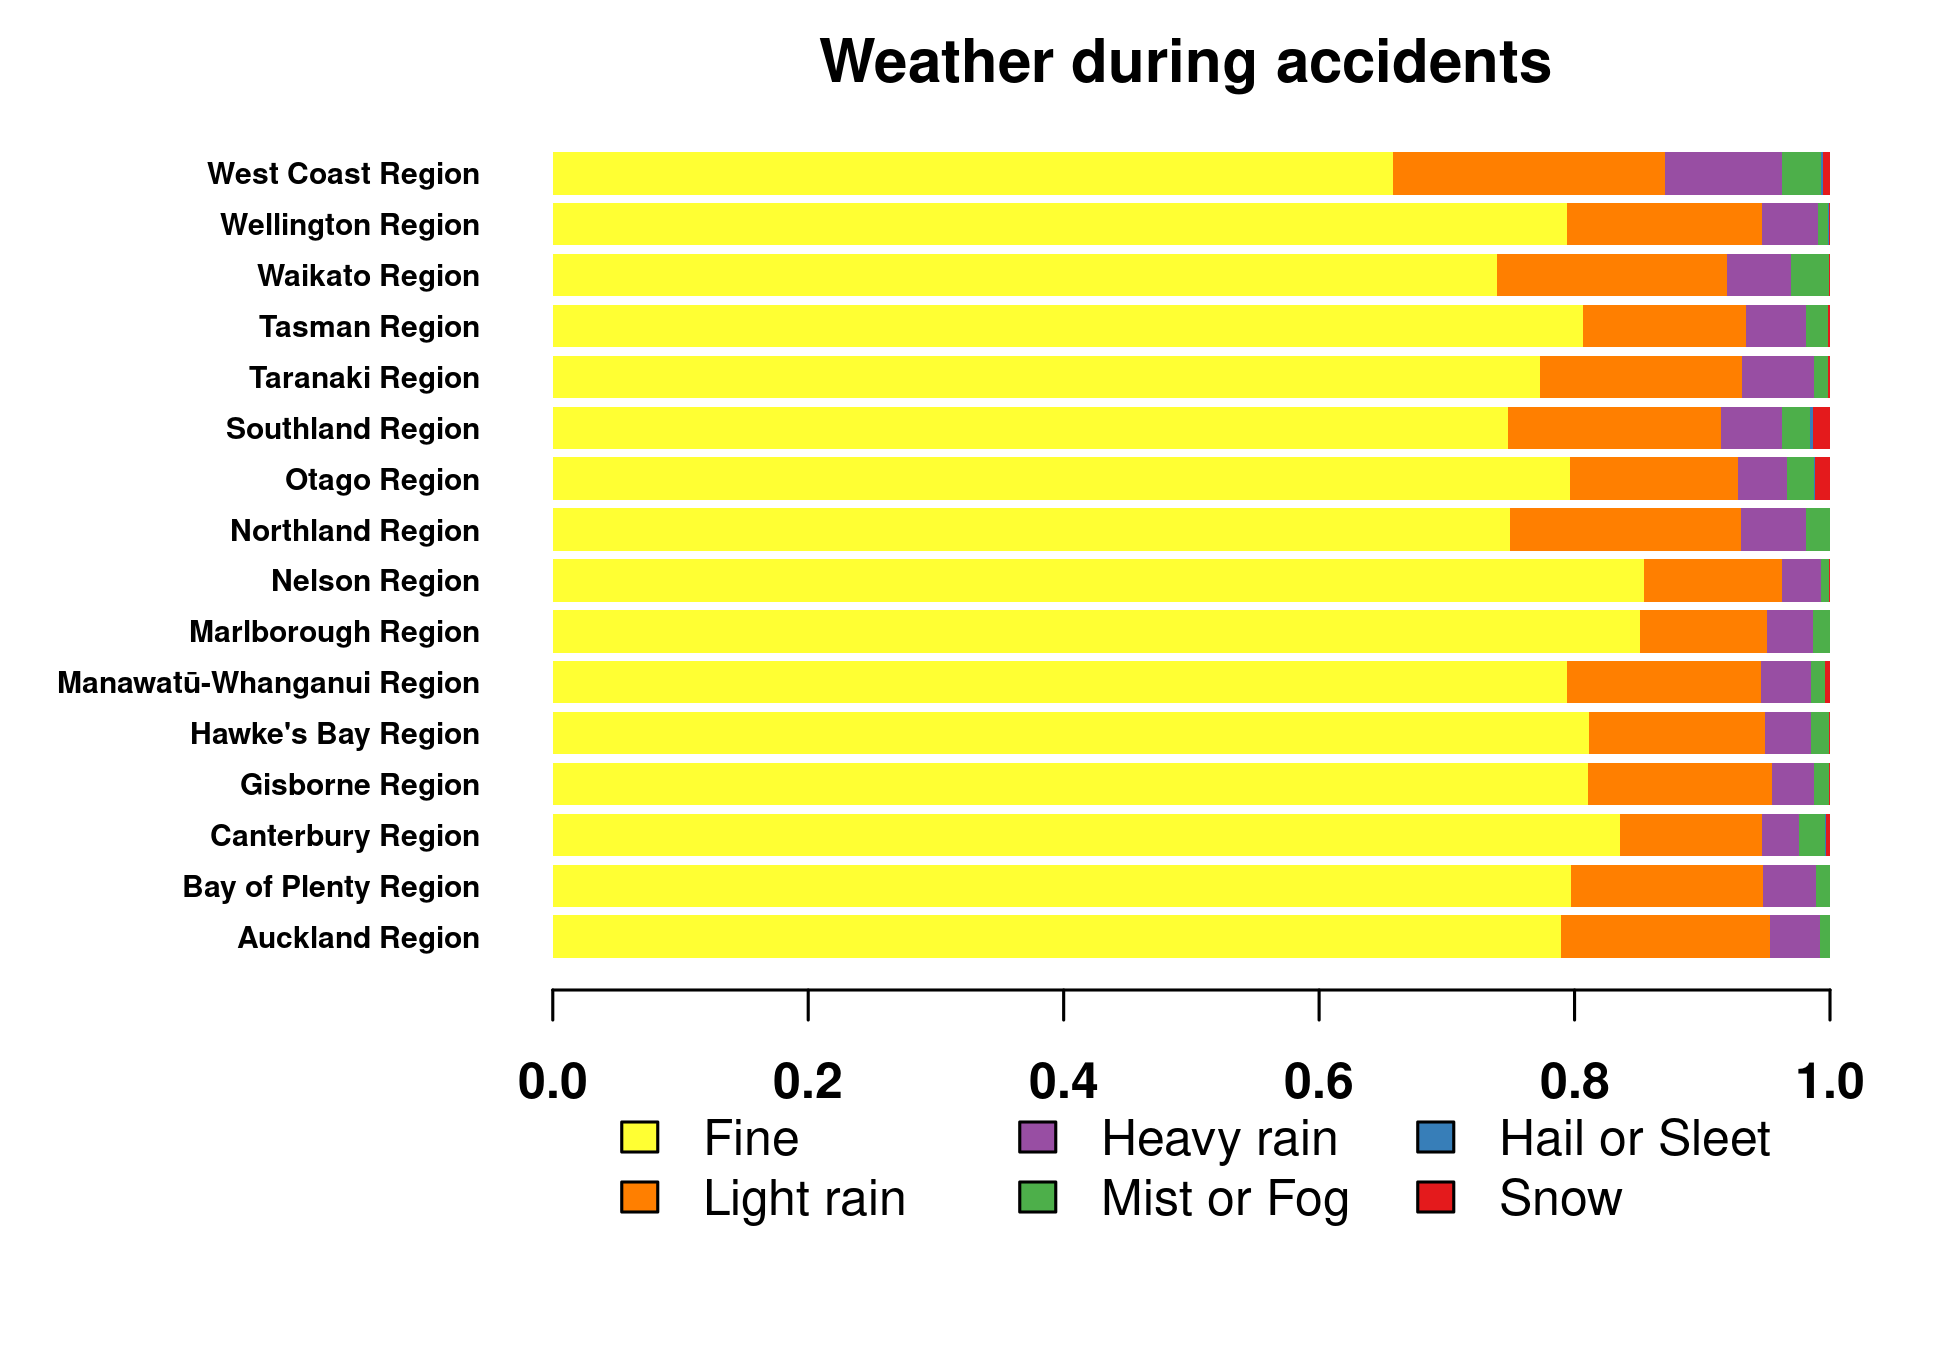
\includegraphics[width=1\textwidth]{figures/regions3-1.png}
\end{frame}

\end{document}
